% Options for packages loaded elsewhere
\PassOptionsToPackage{unicode}{hyperref}
\PassOptionsToPackage{hyphens}{url}
%
\documentclass[
]{article}
\usepackage{amsmath,amssymb}
\usepackage{iftex}
\ifPDFTeX
  \usepackage[T1]{fontenc}
  \usepackage[utf8]{inputenc}
  \usepackage{textcomp} % provide euro and other symbols
\else % if luatex or xetex
  \usepackage{unicode-math} % this also loads fontspec
  \defaultfontfeatures{Scale=MatchLowercase}
  \defaultfontfeatures[\rmfamily]{Ligatures=TeX,Scale=1}
\fi
\usepackage{lmodern}
\ifPDFTeX\else
  % xetex/luatex font selection
\fi
% Use upquote if available, for straight quotes in verbatim environments
\IfFileExists{upquote.sty}{\usepackage{upquote}}{}
\IfFileExists{microtype.sty}{% use microtype if available
  \usepackage[]{microtype}
  \UseMicrotypeSet[protrusion]{basicmath} % disable protrusion for tt fonts
}{}
\makeatletter
\@ifundefined{KOMAClassName}{% if non-KOMA class
  \IfFileExists{parskip.sty}{%
    \usepackage{parskip}
  }{% else
    \setlength{\parindent}{0pt}
    \setlength{\parskip}{6pt plus 2pt minus 1pt}}
}{% if KOMA class
  \KOMAoptions{parskip=half}}
\makeatother
\usepackage{xcolor}
\usepackage[margin=1in]{geometry}
\usepackage{color}
\usepackage{fancyvrb}
\newcommand{\VerbBar}{|}
\newcommand{\VERB}{\Verb[commandchars=\\\{\}]}
\DefineVerbatimEnvironment{Highlighting}{Verbatim}{commandchars=\\\{\}}
% Add ',fontsize=\small' for more characters per line
\usepackage{framed}
\definecolor{shadecolor}{RGB}{248,248,248}
\newenvironment{Shaded}{\begin{snugshade}}{\end{snugshade}}
\newcommand{\AlertTok}[1]{\textcolor[rgb]{0.94,0.16,0.16}{#1}}
\newcommand{\AnnotationTok}[1]{\textcolor[rgb]{0.56,0.35,0.01}{\textbf{\textit{#1}}}}
\newcommand{\AttributeTok}[1]{\textcolor[rgb]{0.13,0.29,0.53}{#1}}
\newcommand{\BaseNTok}[1]{\textcolor[rgb]{0.00,0.00,0.81}{#1}}
\newcommand{\BuiltInTok}[1]{#1}
\newcommand{\CharTok}[1]{\textcolor[rgb]{0.31,0.60,0.02}{#1}}
\newcommand{\CommentTok}[1]{\textcolor[rgb]{0.56,0.35,0.01}{\textit{#1}}}
\newcommand{\CommentVarTok}[1]{\textcolor[rgb]{0.56,0.35,0.01}{\textbf{\textit{#1}}}}
\newcommand{\ConstantTok}[1]{\textcolor[rgb]{0.56,0.35,0.01}{#1}}
\newcommand{\ControlFlowTok}[1]{\textcolor[rgb]{0.13,0.29,0.53}{\textbf{#1}}}
\newcommand{\DataTypeTok}[1]{\textcolor[rgb]{0.13,0.29,0.53}{#1}}
\newcommand{\DecValTok}[1]{\textcolor[rgb]{0.00,0.00,0.81}{#1}}
\newcommand{\DocumentationTok}[1]{\textcolor[rgb]{0.56,0.35,0.01}{\textbf{\textit{#1}}}}
\newcommand{\ErrorTok}[1]{\textcolor[rgb]{0.64,0.00,0.00}{\textbf{#1}}}
\newcommand{\ExtensionTok}[1]{#1}
\newcommand{\FloatTok}[1]{\textcolor[rgb]{0.00,0.00,0.81}{#1}}
\newcommand{\FunctionTok}[1]{\textcolor[rgb]{0.13,0.29,0.53}{\textbf{#1}}}
\newcommand{\ImportTok}[1]{#1}
\newcommand{\InformationTok}[1]{\textcolor[rgb]{0.56,0.35,0.01}{\textbf{\textit{#1}}}}
\newcommand{\KeywordTok}[1]{\textcolor[rgb]{0.13,0.29,0.53}{\textbf{#1}}}
\newcommand{\NormalTok}[1]{#1}
\newcommand{\OperatorTok}[1]{\textcolor[rgb]{0.81,0.36,0.00}{\textbf{#1}}}
\newcommand{\OtherTok}[1]{\textcolor[rgb]{0.56,0.35,0.01}{#1}}
\newcommand{\PreprocessorTok}[1]{\textcolor[rgb]{0.56,0.35,0.01}{\textit{#1}}}
\newcommand{\RegionMarkerTok}[1]{#1}
\newcommand{\SpecialCharTok}[1]{\textcolor[rgb]{0.81,0.36,0.00}{\textbf{#1}}}
\newcommand{\SpecialStringTok}[1]{\textcolor[rgb]{0.31,0.60,0.02}{#1}}
\newcommand{\StringTok}[1]{\textcolor[rgb]{0.31,0.60,0.02}{#1}}
\newcommand{\VariableTok}[1]{\textcolor[rgb]{0.00,0.00,0.00}{#1}}
\newcommand{\VerbatimStringTok}[1]{\textcolor[rgb]{0.31,0.60,0.02}{#1}}
\newcommand{\WarningTok}[1]{\textcolor[rgb]{0.56,0.35,0.01}{\textbf{\textit{#1}}}}
\usepackage{longtable,booktabs,array}
\usepackage{calc} % for calculating minipage widths
% Correct order of tables after \paragraph or \subparagraph
\usepackage{etoolbox}
\makeatletter
\patchcmd\longtable{\par}{\if@noskipsec\mbox{}\fi\par}{}{}
\makeatother
% Allow footnotes in longtable head/foot
\IfFileExists{footnotehyper.sty}{\usepackage{footnotehyper}}{\usepackage{footnote}}
\makesavenoteenv{longtable}
\usepackage{graphicx}
\makeatletter
\def\maxwidth{\ifdim\Gin@nat@width>\linewidth\linewidth\else\Gin@nat@width\fi}
\def\maxheight{\ifdim\Gin@nat@height>\textheight\textheight\else\Gin@nat@height\fi}
\makeatother
% Scale images if necessary, so that they will not overflow the page
% margins by default, and it is still possible to overwrite the defaults
% using explicit options in \includegraphics[width, height, ...]{}
\setkeys{Gin}{width=\maxwidth,height=\maxheight,keepaspectratio}
% Set default figure placement to htbp
\makeatletter
\def\fps@figure{htbp}
\makeatother
\setlength{\emergencystretch}{3em} % prevent overfull lines
\providecommand{\tightlist}{%
  \setlength{\itemsep}{0pt}\setlength{\parskip}{0pt}}
\setcounter{secnumdepth}{5}
\newlength{\cslhangindent}
\setlength{\cslhangindent}{1.5em}
\newlength{\csllabelwidth}
\setlength{\csllabelwidth}{3em}
\newlength{\cslentryspacingunit} % times entry-spacing
\setlength{\cslentryspacingunit}{\parskip}
\newenvironment{CSLReferences}[2] % #1 hanging-ident, #2 entry spacing
 {% don't indent paragraphs
  \setlength{\parindent}{0pt}
  % turn on hanging indent if param 1 is 1
  \ifodd #1
  \let\oldpar\par
  \def\par{\hangindent=\cslhangindent\oldpar}
  \fi
  % set entry spacing
  \setlength{\parskip}{#2\cslentryspacingunit}
 }%
 {}
\usepackage{calc}
\newcommand{\CSLBlock}[1]{#1\hfill\break}
\newcommand{\CSLLeftMargin}[1]{\parbox[t]{\csllabelwidth}{#1}}
\newcommand{\CSLRightInline}[1]{\parbox[t]{\linewidth - \csllabelwidth}{#1}\break}
\newcommand{\CSLIndent}[1]{\hspace{\cslhangindent}#1}
% Load necessary packages
\usepackage{amsmath}    % For advanced math typesetting
\usepackage{graphicx}   % For including images
\usepackage{hyperref}   % For hyperlinks
\usepackage{geometry}   % For setting page dimensions
\usepackage{fancyhdr}   % For custom headers and footers
\usepackage{setspace}   % For setting line spacing

% Set page dimensions
\geometry{
  a4paper,
  left=25mm,
  right=25mm,
  top=25mm,
  bottom=25mm
}

% Custom header and footer
\pagestyle{fancy}
\fancyhf{}
\fancyhead[L]{\leftmark}
\fancyhead[R]{\thepage}

% Custom commands
\newcommand{\HRule}{\rule{\linewidth}{0.5mm}}

% Set line spacing
\setstretch{1.5}

% Additional settings
\hypersetup{
  colorlinks=true,
  linkcolor=blue,
  filecolor=magenta,
  urlcolor=cyan,
  pdftitle={Your Document Title},
  pdfpagemode=FullScreen,
}
\ifLuaTeX
  \usepackage{selnolig}  % disable illegal ligatures
\fi
\IfFileExists{bookmark.sty}{\usepackage{bookmark}}{\usepackage{hyperref}}
\IfFileExists{xurl.sty}{\usepackage{xurl}}{} % add URL line breaks if available
\urlstyle{same}
\hypersetup{
  pdftitle={Lecture 7: The Relationship Between Correlation and Regression},
  hidelinks,
  pdfcreator={LaTeX via pandoc}}

\title{Lecture 7: The Relationship Between Correlation and Regression}
\usepackage{etoolbox}
\makeatletter
\providecommand{\subtitle}[1]{% add subtitle to \maketitle
  \apptocmd{\@title}{\par {\large #1 \par}}{}{}
}
\makeatother
\subtitle{C91AR: Advanced Statistics using R}
\author{}
\date{\vspace{-2.5em}2025-03-04}

\begin{document}
\maketitle

{
\setcounter{tocdepth}{2}
\tableofcontents
}
\hypertarget{reading-for-today}{%
\section{Reading for today}\label{reading-for-today}}

Barr (2025)

Canduela and Raeside (2020)

\hypertarget{session-outline}{%
\section{Session outline}\label{session-outline}}

\begin{itemize}
\tightlist
\item
  Today, we are continuing to learn about statistics through data
  simulation.
\item
  We also continue to use the ``heights\_and\_weights.csv'' dataset we
  used for the session on simulating correlation data.
\item
  We are moving on to look at how you can estimate values given the
  statistics of simple regression.
\end{itemize}

\hypertarget{regression-theory}{%
\section{Regression Theory}\label{regression-theory}}

\begin{itemize}
\tightlist
\item
  Regression can be thought of as a process of generating a line of best
  fit given the data.
\item
  Rather than draw by hand, a procedure called \textbf{least squares
  regression} can be used to reliably draw this line.
\end{itemize}

\hypertarget{least-squares-regression}{%
\subsection{Least squares regression}\label{least-squares-regression}}

The line is adjusted to minimise the SSE (sum of squared deviations;
\(e_{i}^{2}\)) of each point from the line:

Minimise SSE =
\(min \underset{i=1}{\stackrel{n}{\sum}}e_{i}^{2} = min \underset{i=1}{\stackrel{n}{\sum}}(y_{i} - \hat{y}_{i})^2\)

\begin{itemize}
\tightlist
\item
  \(y_{i}\) = observed value
\item
  \(\hat{y}_{i}\) = predicted value
\item
  \(e_{i}\) = error
\item
  \(n\) = number of observations
\item
  \(\underset{i=1}{\stackrel{n}{\sum}}\) = summation of a sequence of
  terms indexed by \(i\), starting from \(i = 1\) and ending at
  \(i = n\)
\end{itemize}

\hypertarget{illustration-of-regression}{%
\section{Illustration of regression}\label{illustration-of-regression}}

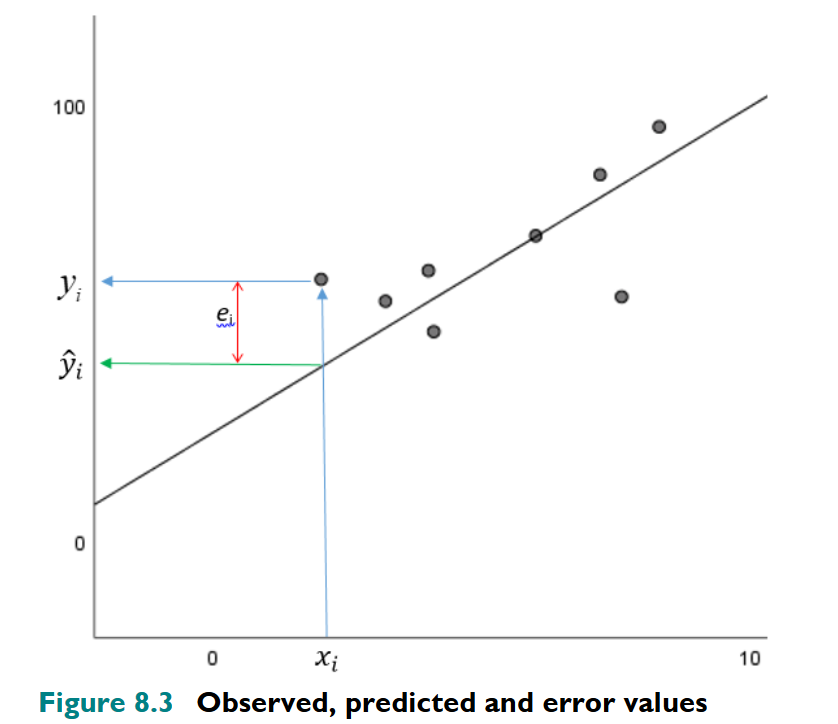
\includegraphics[width=6.04167in,height=6.14583in]{images/RM3_regression.png}

\begin{itemize}
\tightlist
\item
  So, least squares regression is summation of all of the squared
  differences (\(e_{i}\)) between the observed (\(y_{i}\)) and predicted
  (\(\hat{y}_{i}\)) values of \(y\)
\end{itemize}

\hypertarget{regression-formula}{%
\section{Regression formula}\label{regression-formula}}

\[Y_i = \beta_0 + \beta_1 X_i + e_i\]

Where\ldots{}

\begin{itemize}
\tightlist
\item
  \(y_{i}\) = \(i\)th observation of the dependent variable,
  \(i = 1,2,...,n\)
\item
  \(x_{i}\) = \(i\)th observation for the independent variable,
  \(i = 1,2,...n\)
\item
  \(\beta_{0}\) = intercept or constant
\item
  \(\beta_{1}\) = the slope or gradient of the predictor/independent
  variable
\item
  \(\epsilon_{i}\) = error or residual of the \(i\)th observation
\item
  \(n\) = total number of observations
\end{itemize}

\hypertarget{the-relationship-between-correlation-and-regression}{%
\section{The relationship between correlation and
regression?}\label{the-relationship-between-correlation-and-regression}}

\begin{itemize}
\tightlist
\item
  Correlation tells us about the strength and relationship between two
  variables.
\item
  Regression (on the other hand) predicts the value of one variable
  based on the value of another variable.
\item
  For example, in the heights and weights data, we can use regression
  modelling to \emph{predict someone's weight given their height}.
\end{itemize}

\hypertarget{reproducibility-notation}{%
\section{Reproducibility \& notation}\label{reproducibility-notation}}

\begin{Shaded}
\begin{Highlighting}[]
\CommentTok{\# Set seed for reproducibility}
\FunctionTok{set.seed}\NormalTok{(}\DecValTok{123}\NormalTok{)}

\CommentTok{\# Change the output format}
\FunctionTok{options}\NormalTok{(}\AttributeTok{scipen =} \DecValTok{999}\NormalTok{)}
\end{Highlighting}
\end{Shaded}

\hypertarget{load-packages}{%
\section{Load packages}\label{load-packages}}

\begin{Shaded}
\begin{Highlighting}[]
\CommentTok{\# Load packages}
\NormalTok{pacman}\SpecialCharTok{::}\FunctionTok{p\_load}\NormalTok{(tidyverse,}
\NormalTok{               corrr,}
\NormalTok{               tidyplots)}
\end{Highlighting}
\end{Shaded}

\hypertarget{data-setup}{%
\section{Data setup}\label{data-setup}}

\begin{Shaded}
\begin{Highlighting}[]
\CommentTok{\# Read in the data}
\NormalTok{handw }\OtherTok{\textless{}{-}}
  \FunctionTok{read\_csv}\NormalTok{(}\StringTok{"data\_raw/heights\_and\_weights.csv"}\NormalTok{,}
           \AttributeTok{col\_types =} \StringTok{"dd"}\NormalTok{)}


\CommentTok{\# Add log transformed vectors to dataset}
\NormalTok{handw\_log }\OtherTok{\textless{}{-}}
\NormalTok{  handw }\SpecialCharTok{|\textgreater{}}
  \FunctionTok{mutate}\NormalTok{(}\AttributeTok{hlog =} \FunctionTok{log}\NormalTok{(height\_in),  }
         \AttributeTok{wlog =} \FunctionTok{log}\NormalTok{(weight\_lbs))}
\end{Highlighting}
\end{Shaded}

\hypertarget{remind-me-why-are-we-using-the-log-of-the-data}{%
\section{Remind me, why are we using the log of the
data?}\label{remind-me-why-are-we-using-the-log-of-the-data}}

\hypertarget{raw-data}{%
\section{Raw data}\label{raw-data}}

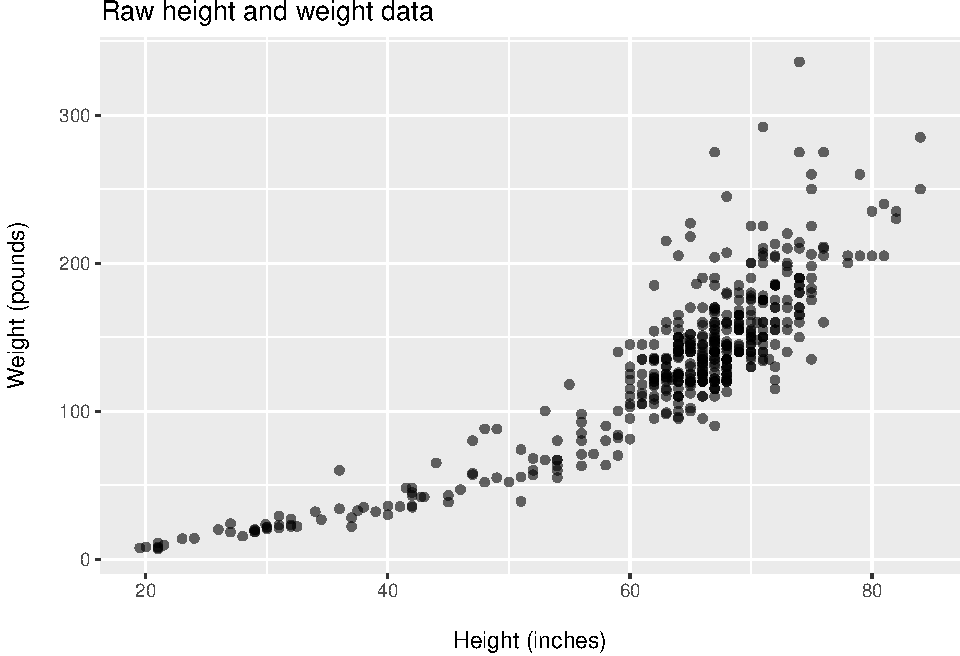
\includegraphics{L7_Correlation_and_regression_pdf_files/figure-latex/unnamed-chunk-4-1.pdf}

\hypertarget{normalised-data}{%
\section{Normalised data}\label{normalised-data}}

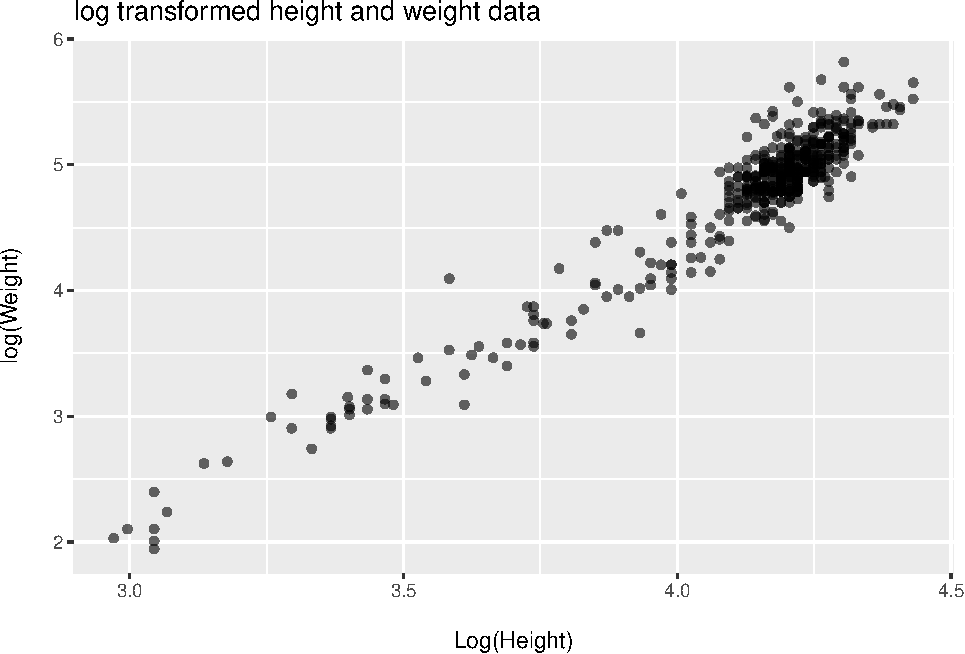
\includegraphics{L7_Correlation_and_regression_pdf_files/figure-latex/unnamed-chunk-5-1.pdf}

\hypertarget{rationale-for-taking-the-log}{%
\section{Rationale for taking the
log}\label{rationale-for-taking-the-log}}

\begin{itemize}
\tightlist
\item
  When we take the log of the data we normalise it, to stabilise the
  variance in our vectors.
\item
  This is particularly useful if the data are highly skewed or show
  \textbf{heteroscedasticity}

  \begin{itemize}
  \tightlist
  \item
    When the difference between the observed and predicted values (i.e.,
    the residuals \(e_i\)) is not constant across all levels of the
    independent variables.
  \item
    For the heights and weights data, you can see that the residuals
    increase as the values for height and weight approach the upper
    limit
  \end{itemize}
\item
  Normalised data is more suitable for statistical analysis that assume
  normality, such as linear regression.
\end{itemize}

\hypertarget{using-regression-to-make-predictions-based-on-height-and-weight-data}{%
\section{Using regression to make predictions based on height and weight
data}\label{using-regression-to-make-predictions-based-on-height-and-weight-data}}

\textbf{Regression formula}

\[Y_i = \beta_0 + \beta_1 X_i + e_i\]

\textbf{In the context of predicting height from weight}

\begin{itemize}
\item
  \(Y_i\) = prediction of a person \(i\)'s weight
\item
  \(X_i\) = observed height
\item
  \(\beta_0\) = y-intercept
\item
  \(\beta_1\) = slope parameter
\item
  \(e_i\) = residuals

  \begin{itemize}
  \tightlist
  \item
    Note, it is assumed that \(e_i\) comes from a normal distribution
    with a mean of zero and variance \(\sigma^2\).
  \end{itemize}
\end{itemize}

\hypertarget{making-predictions-using-the-available-statistics}{%
\section{Making predictions using the available
statistics}\label{making-predictions-using-the-available-statistics}}

To estimate the parameters of the regression between the y-intercept
(\(\beta_0\)) and the slope (\(\beta_1\)) all we need is the:

\begin{itemize}
\tightlist
\item
  Mean estimates for \(X\) and \(Y\), denoted as \(\hat{\mu_x}\) \&
  \(\hat{\mu_y}\)
\item
  Standard deviations for \(X\) and \(Y\), denoted as \(\hat{\sigma_x}\)
  \& \(\hat{\sigma_y}\)
\item
  Correlations between \(X\) and \(Y\), denoted as \(\hat{\rho}\)
\item
  Note: the \(\hat{hat}\) denotes an estimate of a population parameter.
\end{itemize}

So, the statistics required to estimate \(\beta_0\) and \(\beta_1\) are
much the same as we used for simulating correlational data.

\hypertarget{a-reminder-of-our-previous-calculations}{%
\section{A reminder of our previous
calculations}\label{a-reminder-of-our-previous-calculations}}

\begin{itemize}
\item
  \(\hat{\mu_x} = 4.11, \hat{\sigma_x} = 0.26\) (estimated mean and SD
  of log height)
\item
  \(\hat{\mu_y} = 4.74, \hat{\sigma_y} = 0.65\) (estimated mean and SD
  of log weight)
\item
  \(\hat{\rho_{xy}} = 0.96\) (estimated correlation between the two)
\end{itemize}

\hypertarget{estimating-the-slope-beta_1}{%
\section{\texorpdfstring{Estimating the slope
\(\beta_1\)}{Estimating the slope \textbackslash beta\_1}}\label{estimating-the-slope-beta_1}}

\begin{itemize}
\tightlist
\item
  Let's start by estimating the value of the slope \(\beta_1\).
\item
  Importantly, \(\beta_1\) can be expressed in terms of the correlation
  coefficient \(\rho\) times the ratio of the standard deviations of
  \(Y\) and \(X\).
\end{itemize}

\[\beta_1 = \rho\frac{ \sigma_Y}{\sigma_X}\]

\hypertarget{plugging-in-the-numbers}{%
\section{Plugging in the numbers}\label{plugging-in-the-numbers}}

\begin{itemize}
\tightlist
\item
  Now, you can use the estimates of log height and log weight, to
  estimate the slope:
\end{itemize}

\[\beta_1 = \rho\frac{ \sigma_Y}{\sigma_X}\]

In R Code:

\begin{Shaded}
\begin{Highlighting}[]
\CommentTok{\# Estimate slope using formula}
\NormalTok{b1 }\OtherTok{\textless{}{-}}\NormalTok{ .}\DecValTok{96} \SpecialCharTok{*}\NormalTok{ (.}\DecValTok{65} \SpecialCharTok{/}\NormalTok{ .}\DecValTok{26}\NormalTok{)}
\NormalTok{b1 }\CommentTok{\# 2.4}
\end{Highlighting}
\end{Shaded}

\begin{verbatim}
## [1] 2.4
\end{verbatim}

\hypertarget{using-the-axis-to-fill-in-the-blanks-part-1}{%
\section{Using the Axis to fill in the blanks: part
1}\label{using-the-axis-to-fill-in-the-blanks-part-1}}

\begin{itemize}
\item
  For mathematical reasons, the regression line is \textbf{guaranteed to
  go through the point corresponding to the mean of both \(X\) and
  \(Y\), i.e., the point (\(\mu_x\), \(\mu_y\))}.
\item
  One way to think about this is that the regression line pivots around
  that point depending on the slope (\(\beta_1\)).
\item
  We also know that \(\beta_0\) is the y-intercept, where the line
  crosses the vertical axis at \(X\) = 0.
\end{itemize}

\hypertarget{regression-line-passing-through-variable-means-mu_x-mu_y}{%
\section{\texorpdfstring{Regression line passing through variable means
(\(\mu_x\),
\(\mu_y\))}{Regression line passing through variable means (\textbackslash mu\_x, \textbackslash mu\_y)}}\label{regression-line-passing-through-variable-means-mu_x-mu_y}}

\begin{verbatim}
## Warning in geom_point(aes(x = mean_hlog, y = mean_wlog), color = "purple", : All aesthetics have length 1, but the data has 475 rows.
## i Please consider using `annotate()` or provide this layer with data containing
##   a single row.
\end{verbatim}

\begin{verbatim}
## `geom_smooth()` using formula = 'y ~ x'
\end{verbatim}

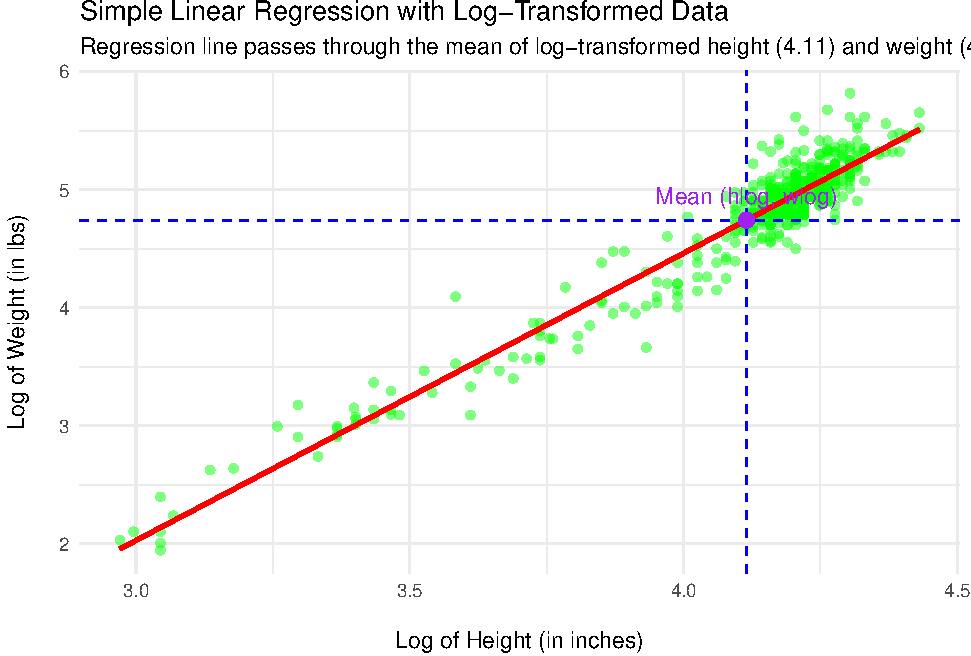
\includegraphics{L7_Correlation_and_regression_pdf_files/figure-latex/unnamed-chunk-6-1.pdf}

\hypertarget{using-the-axis-to-fill-in-the-blanks-part-2}{%
\section{Using the Axis to fill in the blanks: part
2}\label{using-the-axis-to-fill-in-the-blanks-part-2}}

\begin{itemize}
\item
  From all of this information we can calculate \(\beta_0\).
\item
  Remember that \(\beta_1\) tells you that for each change in \(X\) you
  have a corresponding change of \textbf{2.4} for \(Y\), and that the
  line goes through points (\(\mu_x\), \(\mu_y\)) as well as the
  y-intercept (0, \(\beta_0\)).
\end{itemize}

\hypertarget{re-framing-the-calculations}{%
\section{Re-framing the
calculations}\label{re-framing-the-calculations}}

\begin{itemize}
\item
  Think about stepping back unit-by-unit from the mean of \(X = \mu_x\)
  to \(X = 0\).
\item
  At \(X =\mu_x\), \(Y = 4.74\), because as stated earlier, the
  regression line is guaranteed to go through the point corresponding to
  the mean of both \(X\) and \(Y\), i.e., the point (\(\mu_x\),
  \(\mu_y\)) or (4.11, 4.74).
\item
  Each unit step you take backward in the \(X\) dimension, \(Y\) will
  reduce by \(\beta_1 = 2.4\) units.
\item
  When you get to zero, \(Y\) will have dropped from \(\mu_y\) to
  \(\mu_y - \mu_x\beta_1\).
\end{itemize}

\hypertarget{illustrating-this-relationship}{%
\section{Illustrating this
relationship}\label{illustrating-this-relationship}}

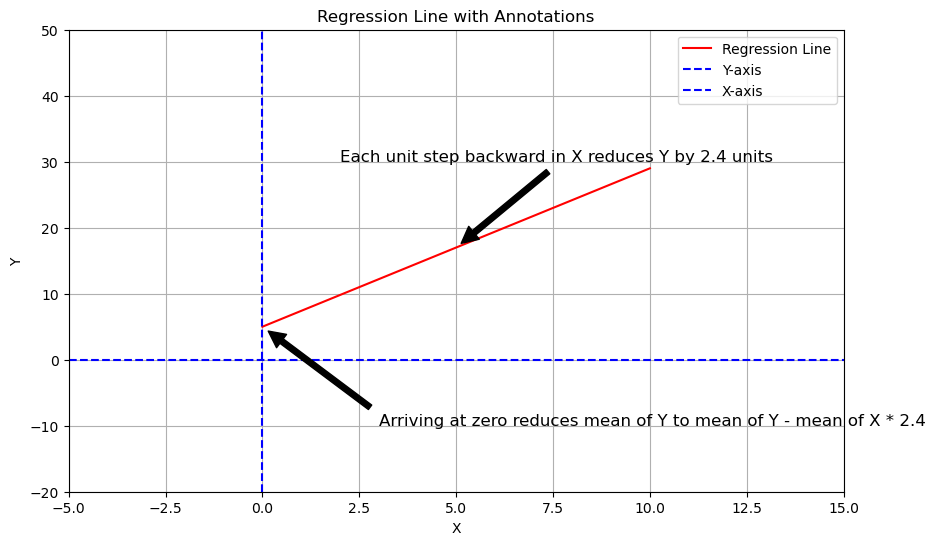
\includegraphics{images/regression_equation.png}

\hypertarget{the-solution}{%
\section{The Solution}\label{the-solution}}

\begin{itemize}
\item
  With all of the above considerations taking into account the solution
  is \(\beta_0 = \mu_y - \mu_x\beta_1\).
\item
  Using this information we can calculate the slope value:
  \(\beta_0 = 4.74 - 4.11 \times 2.4 = -5.124\)
\item
  Now we have the following statistics:

  \begin{itemize}
  \item
    \(\beta_1 = 2.4\)
  \item
    \(\mu_x = 4.11\)
  \item
    \(\mu_y - 4.74\)
  \item
    \(\beta_0 = -5.124\)
  \end{itemize}
\end{itemize}

\hypertarget{plugging-in-the-numbers-1}{%
\section{Plugging in the numbers}\label{plugging-in-the-numbers-1}}

So..

\[Y_i = \beta_0 + \beta_1 X_i + e_i\] Becomes\ldots{}

\[Y_i = -5.124 + 2.4X_i + e_i\]

\hypertarget{checking-the-results}{%
\section{Checking the results}\label{checking-the-results}}

\begin{itemize}
\tightlist
\item
  To check the results, let's first run a regression on the log
  transformed data using \texttt{lm()}, which estimates parameters using
  \emph{ordinary least squares (OLS) regression}.
\item
  In OLS regression, the goal is to find the line that best fits the
  data by minimizing the sum of the squared differences between the
  observed values of the dependent variable and the values predicted by
  the regression line.
\item
  Note, you are interested in the \texttt{Estimate} values.
\end{itemize}

\begin{Shaded}
\begin{Highlighting}[]
\FunctionTok{summary}\NormalTok{(}\FunctionTok{lm}\NormalTok{(wlog }\SpecialCharTok{\textasciitilde{}}\NormalTok{ hlog,}
           \AttributeTok{data =}\NormalTok{ handw\_log))}
\end{Highlighting}
\end{Shaded}

\begin{verbatim}
## 
## Call:
## lm(formula = wlog ~ hlog, data = handw_log)
## 
## Residuals:
##      Min       1Q   Median       3Q      Max 
## -0.63296 -0.09915 -0.01366  0.09285  0.65635 
## 
## Coefficients:
##             Estimate Std. Error t value            Pr(>|t|)    
## (Intercept) -5.26977    0.13169  -40.02 <0.0000000000000002 ***
## hlog         2.43304    0.03194   76.17 <0.0000000000000002 ***
## ---
## Signif. codes:  0 '***' 0.001 '**' 0.01 '*' 0.05 '.' 0.1 ' ' 1
## 
## Residual standard error: 0.1774 on 473 degrees of freedom
## Multiple R-squared:  0.9246, Adjusted R-squared:  0.9245 
## F-statistic:  5802 on 1 and 473 DF,  p-value: < 0.00000000000000022
\end{verbatim}

\hypertarget{matching-the-regression-output-to-our-calculations}{%
\section{Matching the regression output to our
calculations}\label{matching-the-regression-output-to-our-calculations}}

From the model output:

\begin{itemize}
\item
  Estimated slope parameter \(\beta_1 = 2.433\) (2.4 from our
  calculations)
\item
  Estimated y-intercept \(\beta_0 = -5.269\) (-5.124 from our
  calculations)
\item
  These don't match exactly because of the rounding we've used in our
  calculations.
\end{itemize}

\hypertarget{checking-your-regression-estimate-with-a-plot}{%
\section{Checking your regression estimate with a
plot}\label{checking-your-regression-estimate-with-a-plot}}

Another way to check the accuracy of your regression calculations is to
superimpose the regression line on the scatter-plot of the log
transformed data.

\begin{Shaded}
\begin{Highlighting}[]
\FunctionTok{ggplot}\NormalTok{(}\AttributeTok{data =}\NormalTok{ handw\_log, }
       \FunctionTok{aes}\NormalTok{(hlog, wlog)) }\SpecialCharTok{+}
  \FunctionTok{geom\_point}\NormalTok{(}\AttributeTok{alpha =}\NormalTok{ .}\DecValTok{3}\NormalTok{)}\SpecialCharTok{+}
  \FunctionTok{geom\_abline}\NormalTok{(}\AttributeTok{intercept =} \SpecialCharTok{{-}}\FloatTok{5.124}\NormalTok{, }
              \AttributeTok{slope =} \FloatTok{2.4}\NormalTok{, }
              \AttributeTok{colour =} \StringTok{\textquotesingle{}purple\textquotesingle{}}\NormalTok{) }\SpecialCharTok{+}
  \FunctionTok{labs}\NormalTok{(}\AttributeTok{title =} \StringTok{"Superimposed regression line onto log transformed data"}\NormalTok{,}
       \AttributeTok{x =} \StringTok{"}\SpecialCharTok{\textbackslash{}n}\StringTok{log(height)"}\NormalTok{, }
       \AttributeTok{y =} \StringTok{"log(weight)}\SpecialCharTok{\textbackslash{}n}\StringTok{"}\NormalTok{)}
\end{Highlighting}
\end{Shaded}

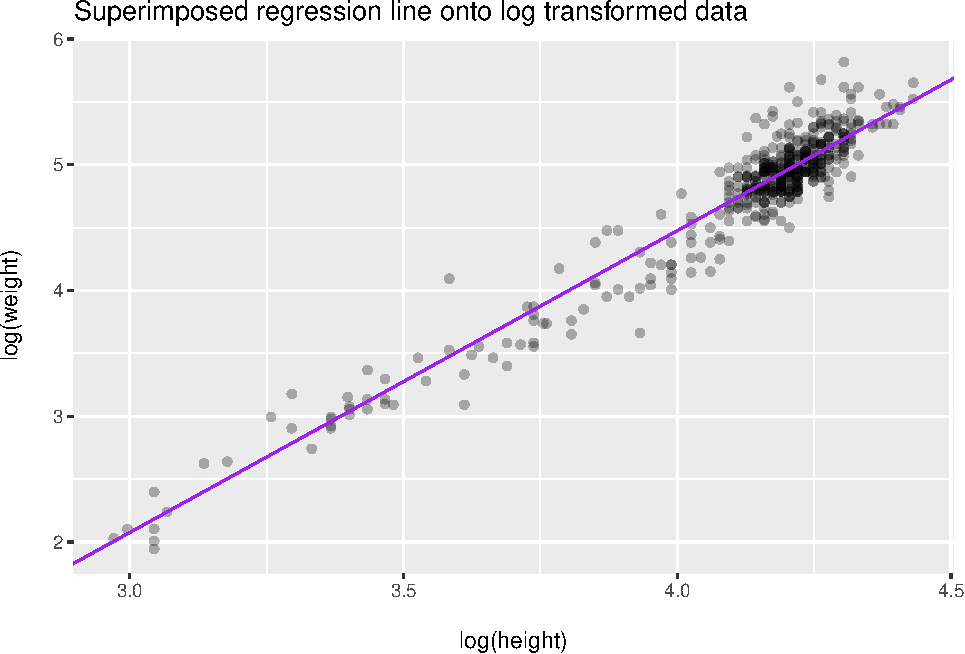
\includegraphics{L7_Correlation_and_regression_pdf_files/figure-latex/unnamed-chunk-9-1.pdf}

\hypertarget{predicting-someones-weight-given-their-height}{%
\section{Predicting someone's weight given their
height}\label{predicting-someones-weight-given-their-height}}

\begin{itemize}
\tightlist
\item
  Say we want to predict the weight of someone who is 69inches or 175cm
  (average height of a person from the US). Let's plug the log of this
  value (4.23) into our regression formula:
\end{itemize}

\(Y_i = -5.124 + 2.4 \times 4.23 + e_i\)

\begin{itemize}
\tightlist
\item
  Note: We do not need to provide the residuals (\(e_i\)) as they are
  estimated from the regression equation.
\end{itemize}

\(Y_i = 5.028\)

\(exp(5.028) = 152.63lbs = 69.2kg\)

\begin{itemize}
\tightlist
\item
  So, our regression model predicts that someone who is 175cm tall would
  weigh 69.2kg.
\end{itemize}

\hypertarget{a-little-more-about-e_i}{%
\section{\texorpdfstring{A little more about
\(e_i\)}{A little more about e\_i}}\label{a-little-more-about-e_i}}

\begin{itemize}
\tightlist
\item
  Conventionally, \(e_i\) come from a normal distribution with
  \(\mu = 0\) and variance \(\sigma^2\).
\item
  \(e_i\) are important for assessing the model's performance and
  diagnostic purposes but they are not necessary for making predictions
  using the regression equation.
\end{itemize}

\hypertarget{model-fit}{%
\section{Model fit}\label{model-fit}}

\begin{itemize}
\tightlist
\item
  We did not cover how to test the model's fit today
\item
  This is covered in the RM3 textbook, and there are good resources
  elsewhere
\item
  I prioritised familiarity with the modelling process over assumption
  checking
\end{itemize}

\hypertarget{roundup}{%
\section{Roundup}\label{roundup}}

\begin{itemize}
\tightlist
\item
  Today I have shown you how to calculate a simple regression model by
  hand using formula
\item
  The aim was to unveil some of the computation that goes on behind the
  scene to help you understand what regression analysis is actually
  doing.
\item
  Using this method, we also made a prediction about someone's height
  given their weight.
\item
  On Monday, we are going to look at multiple regression
\end{itemize}

\hypertarget{r2-coefficient-of-determination}{%
\section{\texorpdfstring{\(R^{2}\) Coefficient of
determination}{R\^{}\{2\} Coefficient of determination}}\label{r2-coefficient-of-determination}}

To this point we have created a regression equation and used it to
predict someone's weight given their height. But, we also want to know
how good a fit our equation is given the data. To calculate this we use
the \textbf{\emph{coefficient of determination}} (\(R^2\)):

\(R^2 = \frac{\text{Sum of Squares Explained by Regression (SSR)}}{\text{Total Sum of Squares (before regression)(TSS)}} = \frac{\underset{i=1}{\stackrel{n}{\sum}}(\hat{y}_{i} - \overline{y})^2}{\underset{i=1}{\stackrel{n}{\sum}}(y_{i} - \overline{y})^{2}}\)

The total variation (TSS) in the dependent variable (weight) is split
into two parts: the part explained (SSR) by the association between the
dependent (weight) and independent (height) variables, and the part that
is unexplained (SSE) since the relationship is never perfect and there
are always some residuals.

\hypertarget{r2-thresholds}{%
\section{\texorpdfstring{\(R^{2}\)
Thresholds}{R\^{}\{2\} Thresholds}}\label{r2-thresholds}}

The higher the \(R^{2}\) value (at least \(70\%\)) the better the model
fit. A reasonable model fit would be more \(R^{2} >= 60\%\).

The coefficient of determination can take values between 0 and 1, but is
commonly reported as a percentage, as it represent the proportion of the
variation in the dependent variable (\(Y_{i}\)) which is explained by
the predictor/independent variable (\(X_{i}\)).

\hypertarget{exploring-the-errors}{%
\section{Exploring the Errors}\label{exploring-the-errors}}

To diagnose the quality of the model further we need to look at the
errors or residuals \((y_{i} - \hat{y}_{i})\) after running the
regression model.

Model residuals should be \textbf{randomly scattered} with \textbf{no
extreme values} and should have a \textbf{mean of zero}.

Should these requirements not be met we would have to further
investigate whether there is information in the residuals that could be
covered by the model or be considered a cause for concern.

A histogram of the residuals and normal probability plot can help you
decide how well your residuals fit into the model.

\hypertarget{histogram-of-model-residuals}{%
\section{Histogram of model
residuals}\label{histogram-of-model-residuals}}

Raw data: residuals plot code

\begin{Shaded}
\begin{Highlighting}[]
\CommentTok{\# Create model for raw data}
\NormalTok{mod1 }\OtherTok{\textless{}{-}}
  \FunctionTok{lm}\NormalTok{(weight\_lbs }\SpecialCharTok{\textasciitilde{}}\NormalTok{ height\_in,}
     \AttributeTok{data =}\NormalTok{ handw)}

\CommentTok{\# Create residuals object}
\NormalTok{residuals\_df }\OtherTok{\textless{}{-}} 
\NormalTok{  mod1}\SpecialCharTok{$}\NormalTok{residuals }\SpecialCharTok{|\textgreater{}}
  \FunctionTok{as\_tibble}\NormalTok{() }\SpecialCharTok{|\textgreater{}}
  \FunctionTok{rename}\NormalTok{(}\AttributeTok{residuals =}\NormalTok{ value)}

\CommentTok{\# Plot the data}
\FunctionTok{ggplot}\NormalTok{(residuals\_df, }\FunctionTok{aes}\NormalTok{(}\AttributeTok{x =}\NormalTok{ residuals)) }\SpecialCharTok{+}
  \FunctionTok{geom\_histogram}\NormalTok{(}\AttributeTok{binwidth =} \DecValTok{10}\NormalTok{) }\SpecialCharTok{+}
  \FunctionTok{labs}\NormalTok{(}\AttributeTok{title =} \StringTok{"Histogram of Residuals"}\NormalTok{,}
       \AttributeTok{x =} \StringTok{"Residuals"}\NormalTok{,}
       \AttributeTok{y =} \StringTok{"Frequency"}\NormalTok{)}
\end{Highlighting}
\end{Shaded}

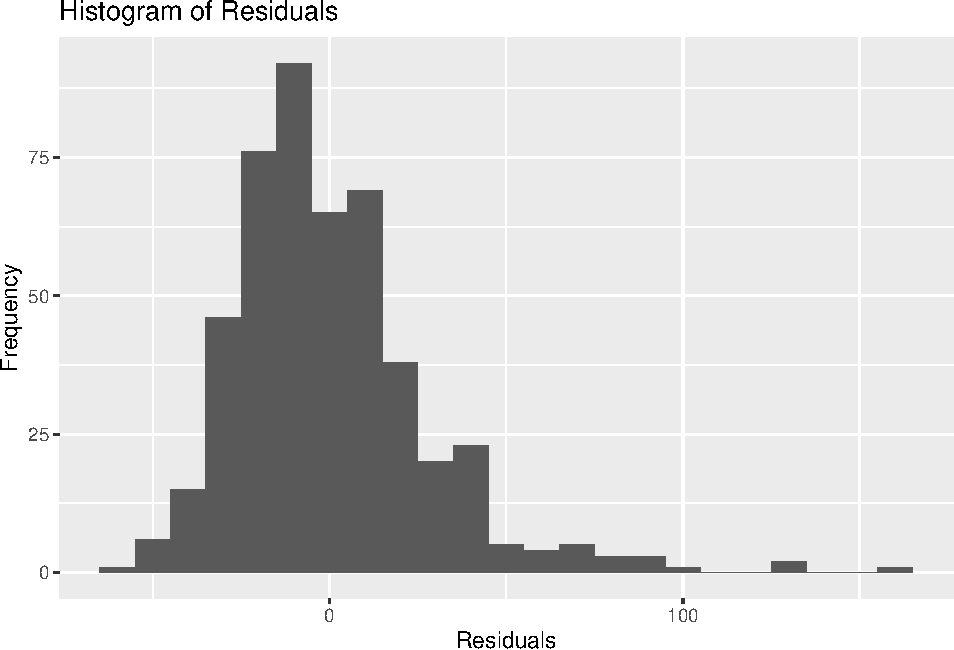
\includegraphics{L7_Correlation_and_regression_pdf_files/figure-latex/unnamed-chunk-10-1.pdf}

\hypertarget{raw-data-residuals-plot-output}{%
\section{Raw data: residuals plot
output}\label{raw-data-residuals-plot-output}}

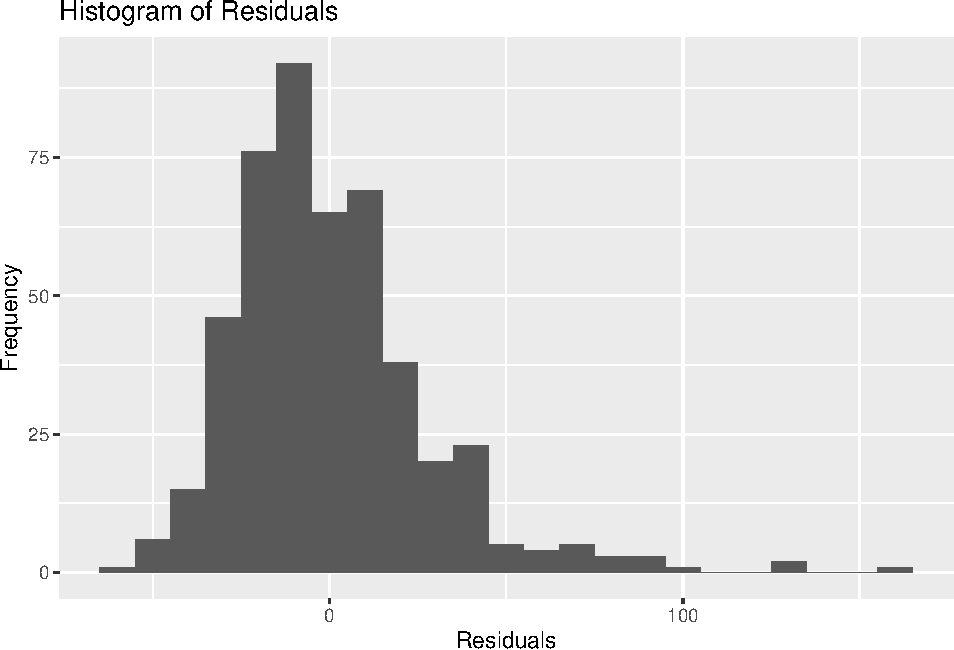
\includegraphics{L7_Correlation_and_regression_pdf_files/figure-latex/unnamed-chunk-11-1.pdf}

\hypertarget{transformed-data-residuals-plot}{%
\section{Transformed data: residuals
plot}\label{transformed-data-residuals-plot}}

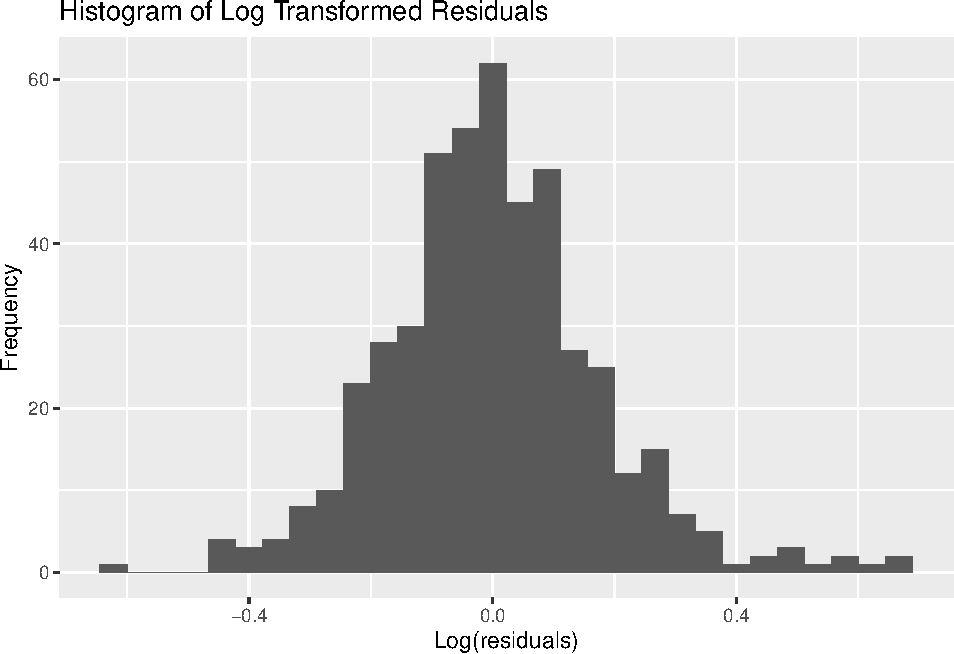
\includegraphics{L7_Correlation_and_regression_pdf_files/figure-latex/unnamed-chunk-12-1.pdf}

\hypertarget{normal-probability-probability-p-p-plots}{%
\section{Normal Probability-Probability (P-P)
Plots}\label{normal-probability-probability-p-p-plots}}

\textbf{Raw data: Normal PP plot code}

\begin{Shaded}
\begin{Highlighting}[]
\CommentTok{\# Extract residuals}
\NormalTok{residuals }\OtherTok{\textless{}{-}}
\NormalTok{  mod1}\SpecialCharTok{$}\NormalTok{residuals}

\CommentTok{\# Calculate theoretical quantiles}
\NormalTok{mod1\_quantiles }\OtherTok{\textless{}{-}}
  \FunctionTok{qqnorm}\NormalTok{(residuals, }\AttributeTok{plot.it =} \ConstantTok{FALSE}\NormalTok{)}\SpecialCharTok{$}\NormalTok{x}

\CommentTok{\# Create a data frame with residuals and theoretical quantiles}
\NormalTok{pp\_df }\OtherTok{\textless{}{-}} 
  \FunctionTok{data.frame}\NormalTok{(}
  \AttributeTok{residuals =}\NormalTok{ residuals,}
  \AttributeTok{theoretical\_quantiles =}\NormalTok{ mod1\_quantiles}
\NormalTok{)}

\CommentTok{\# Plot the P{-}P plot}
\FunctionTok{ggplot}\NormalTok{(pp\_df, }\FunctionTok{aes}\NormalTok{(}\AttributeTok{sample =}\NormalTok{ residuals)) }\SpecialCharTok{+}
  \FunctionTok{stat\_qq}\NormalTok{() }\SpecialCharTok{+}
  \FunctionTok{stat\_qq\_line}\NormalTok{() }\SpecialCharTok{+}
  \FunctionTok{labs}\NormalTok{(}\AttributeTok{title =} \StringTok{"Normal P{-}P Plot of Residuals"}\NormalTok{,}
       \AttributeTok{x =} \StringTok{"Theoretical Quantiles"}\NormalTok{,}
       \AttributeTok{y =} \StringTok{"Sample Quantiles"}\NormalTok{) }\SpecialCharTok{+}
  \FunctionTok{theme\_minimal}\NormalTok{()}
\end{Highlighting}
\end{Shaded}

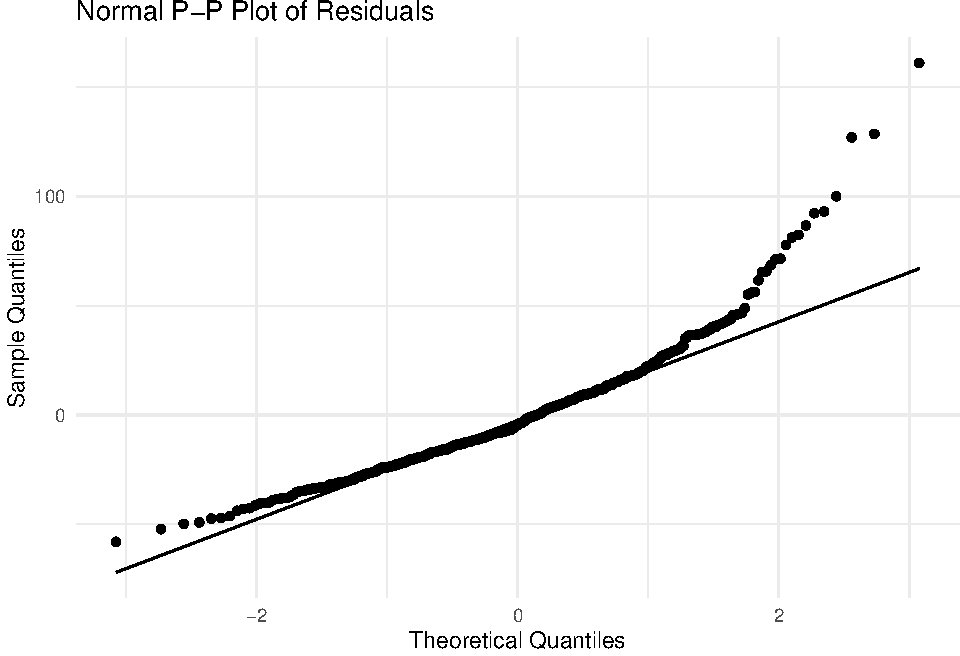
\includegraphics{L7_Correlation_and_regression_pdf_files/figure-latex/unnamed-chunk-13-1.pdf}

\hypertarget{raw-data-normal-pp-plot-output}{%
\section{Raw data: Normal PP plot
output}\label{raw-data-normal-pp-plot-output}}

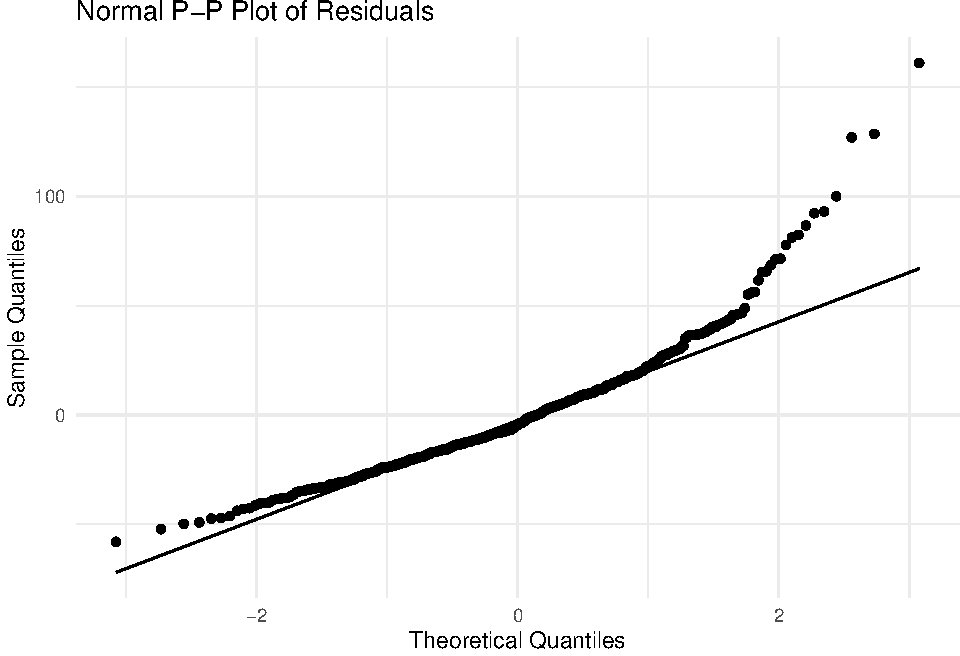
\includegraphics{L7_Correlation_and_regression_pdf_files/figure-latex/unnamed-chunk-14-1.pdf}

\hypertarget{transformed-data-normal-pp-plot-ouput}{%
\section{Transformed data: Normal PP plot
ouput}\label{transformed-data-normal-pp-plot-ouput}}

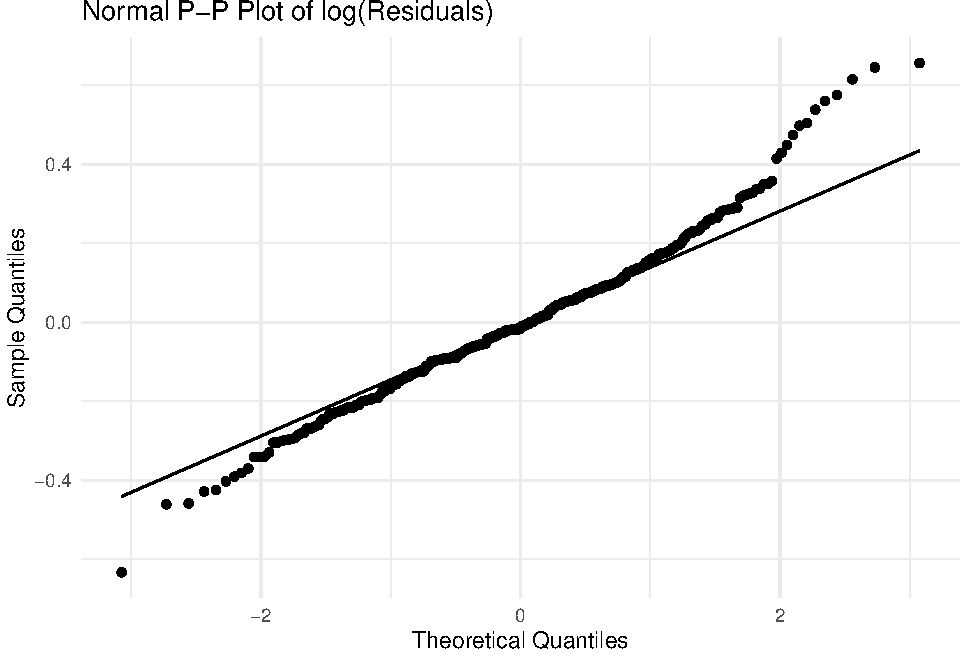
\includegraphics{L7_Correlation_and_regression_pdf_files/figure-latex/unnamed-chunk-15-1.pdf}

\hypertarget{testing-the-significance-of-the-model-and-its-coefficients}{%
\section{Testing the Significance of the model and its
coefficients}\label{testing-the-significance-of-the-model-and-its-coefficients}}

We can use statistical tests to determine how well we are approximating
the population parameters with those in our model. To do this we can use
two methods:

\begin{itemize}
\tightlist
\item
  Analysis of variance (ANOVA): tests overall significance of the model
\item
  \(t\)-test: test the individual significance of the coefficients.
\end{itemize}

\hypertarget{testing-the-overall-significance-of-the-model}{%
\subsection{Testing the overall significance of the
model}\label{testing-the-overall-significance-of-the-model}}

Testing the overall significance of the model evaluates how well the
independent variables reliable predict the dependent variable. We can
create hypotheses to make our statistical inferences:

\(H_{0}\): The regression model does not explain a significant
proportion of the variance in weight (our DV).

VS

\(H_{1}\): The regression model does explain a significant proportion of
the variation in weight.

And we test the above using the \(F\)-distribution.

\hypertarget{anova-for-regression-modelling}{%
\section{ANOVA for regression
modelling}\label{anova-for-regression-modelling}}

\textbf{ANOVA for regression}

\begin{longtable}[]{@{}
  >{\raggedright\arraybackslash}p{(\columnwidth - 8\tabcolsep) * \real{0.1795}}
  >{\raggedright\arraybackslash}p{(\columnwidth - 8\tabcolsep) * \real{0.1880}}
  >{\raggedright\arraybackslash}p{(\columnwidth - 8\tabcolsep) * \real{0.2137}}
  >{\raggedright\arraybackslash}p{(\columnwidth - 8\tabcolsep) * \real{0.1538}}
  >{\raggedright\arraybackslash}p{(\columnwidth - 8\tabcolsep) * \real{0.2650}}@{}}
\toprule\noalign{}
\begin{minipage}[b]{\linewidth}\raggedright
Source of Variation
\end{minipage} & \begin{minipage}[b]{\linewidth}\raggedright
Sum of Squares (SS)
\end{minipage} & \begin{minipage}[b]{\linewidth}\raggedright
Degrees of Freedom (df)
\end{minipage} & \begin{minipage}[b]{\linewidth}\raggedright
Mean Square (MS)
\end{minipage} & \begin{minipage}[b]{\linewidth}\raggedright
F-Statistic (F)
\end{minipage} \\
\midrule\noalign{}
\endhead
\bottomrule\noalign{}
\endlastfoot
Model &
\(\text{SS}_{\text{model}} = \underset{i=1}{\stackrel{n}{\sum}}(\hat{y}_i - \bar{y})^2\)
& \(k\) & \(\text{MSR} = \frac{\text{SSR}}{k}\) &
\(\frac{\text{MSR}}{\text{MSE}}\) \\
Residual &
\(\text{SS}_{\text{residual}} = \underset{i=1}{\stackrel{n}{\sum}}(y_i - \hat{y}_i)^2\)
& \(n - k - 1\) & \(\text{MSE} = \frac{\text{SSE}}{n - k - 1}\) & \\
Total &
\(\text{TSS} = SSR + SSE = \underset{i=1}{\stackrel{n}{\sum}}(y_i - \bar{y})^2\)
& \(n - 1\) & & \\
\end{longtable}

\begin{center}\rule{0.5\linewidth}{0.5pt}\end{center}

ANOVA for regression: key

\begin{itemize}
\tightlist
\item
  \(n\) = total number of observations
\item
  \(k\) = total number of independent variables
\item
  \(y\) = the observed values
\item
  \(\overline{y}\) = mean of the dependent variables
\item
  \(\hat{y}_{i}\) = the estimated values
\end{itemize}

\hypertarget{anova-for-log-transformed-model}{%
\section{ANOVA for log transformed
model}\label{anova-for-log-transformed-model}}

\begin{Shaded}
\begin{Highlighting}[]
\CommentTok{\# Run an ANOVA on our log transformed model}
\NormalTok{anova\_results }\OtherTok{\textless{}{-}}
  \FunctionTok{anova}\NormalTok{(mod2)}

\FunctionTok{print}\NormalTok{(anova\_results)}
\end{Highlighting}
\end{Shaded}

\begin{verbatim}
## Analysis of Variance Table
## 
## Response: wlog
##            Df  Sum Sq Mean Sq F value                Pr(>F)    
## hlog        1 182.622 182.622  5801.8 < 0.00000000000000022 ***
## Residuals 473  14.888   0.031                                  
## ---
## Signif. codes:  0 '***' 0.001 '**' 0.01 '*' 0.05 '.' 0.1 ' ' 1
\end{verbatim}

\begin{center}\rule{0.5\linewidth}{0.5pt}\end{center}

\begin{Shaded}
\begin{Highlighting}[]
\CommentTok{\# Calculate TSS}
\NormalTok{ss\_model }\OtherTok{\textless{}{-}}
\NormalTok{  anova\_results[}\StringTok{"hlog"}\NormalTok{, }\StringTok{"Sum Sq"}\NormalTok{]}

\NormalTok{ss\_residual }\OtherTok{\textless{}{-}}
\NormalTok{  anova\_results[}\StringTok{"Residuals"}\NormalTok{, }\StringTok{"Sum Sq"}\NormalTok{]}

\NormalTok{tss }\OtherTok{\textless{}{-}} 
\NormalTok{  ss\_model }\SpecialCharTok{+}\NormalTok{ ss\_residual}

\FunctionTok{print}\NormalTok{(tss)}
\end{Highlighting}
\end{Shaded}

\begin{verbatim}
## [1] 197.5102
\end{verbatim}

\hypertarget{interpreting-the-results-of-anova}{%
\subsection{Interpreting the results of
ANOVA}\label{interpreting-the-results-of-anova}}

We can see from the output that \texttt{hlog} that the slope of the line
is significant difference from 0, where \(p < 0.001\). Thus we reject
the null hypothesis (\(H_{0}\)).

\hypertarget{references}{%
\section*{References}\label{references}}
\addcontentsline{toc}{section}{References}

\hypertarget{refs}{}
\begin{CSLReferences}{1}{0}
\leavevmode\vadjust pre{\hypertarget{ref-Barr_2025}{}}%
Barr, Dale J. 2025. {``Learning Statistical Models Through Simulation in
r: An Interactive Textbook.''} In \emph{PsyTeachR}, 1.0.0 ed. Creative
Commons. \url{https://psyteachr.github.io/stat-models-v1/}.

\leavevmode\vadjust pre{\hypertarget{ref-Canduela_Raeside_2020}{}}%
Canduela, Jesus, and Robert Raeside. 2020. \emph{The Quantitative
Researcher}. Heriot-Watt University.
\href{https://www.hw.ac.uk/ebs}{www.hw.ac.uk/ebs}.

\end{CSLReferences}

\end{document}
